\chapter{Introduction}

% Current intro sources, mixed together:
% - some new content
% - research statement
% - QED at Large (intro and why proof engineering matters)
% - PUMPKIN Pi
% TODO somewhere, clarify scope of verification here

% TODO can say ``see survey paper''

What would it take to empower programmers of all skill levels across all domains to formally prove
the absence of costly or dangerous bugs in software systems---that is, to formally \intro{verify} them?

Verification has already come a long way toward this since its inception.
This is especially true when it comes to the scale of systems that can be verified.
The seL4~\cite{Klein2009} verified operating system (OS) microkernel, for example,
is the result of a team effort spanning more than
a million lines of proof, costing over 20 person-years.
Given a famous 1977 critique of verification~\cite{DeMillo1977} (emphasis mine):

\begin{quote}
\textit{A sufficiently fanatical researcher}
might be willing to devote \textit{two or 
three years} to verifying a significant 
piece of software if he could be 
assured that the software would remain stable.
\end{quote}
I could argue that, over 40 years, either verification has become easier,
or researchers have become more fanatical. Unfortunately, not all has changed (emphasis still mine):

\begin{quote}
But real-life programs need to 
be maintained and modified. 
There is \intro{no reason to believe} that verifying a modified program is any 
easier than verifying the original the 
first time around.
\end{quote}
This remains so difficult that sometimes, even experts give up in the face of change (Section~\ref{sec:irl}).

This thesis aims to change that by taking advantage of a missed opportunity: tools for developing verified systems (Section~\ref{sec:dev-verif})
have no understanding of how these systems evolve over time, so they miss out on crucial information.
This thesis introduces a new class of verification tools called \textit{proof repair} tools (Section~\ref{sec:thesis})
that understand how software systems evolve, and use the crucial information that evolution carries
to automatically evolve proofs about those systems (Section~\ref{sec:intro-approach}).
Proof repair is \kl{reason to believe} (Section~\ref{sec:intro-results}).

\section{Developing Verified Systems}
\label{sec:dev-verif}

% TODO segue sentence
Proof repair falls under the umbrella of \intro{proof engineering}: the technologies that make it easier
to develop and maintain verified systems (Section~\ref{sec:proofeng}).
Much like software engineering scales programming to large systems, so proof engineering scales verification to large systems. 
In recent years, proof engineers have verified OS microkernels~\cite{Klein2009, Klein2014micro}, machine learning systems~\cite{pmlr-v70-selsam17a}, distributed systems~\cite{Woos:2016:PCF:2854065.2854081}, constraint solvers~\cite{blanchette2018verified}, web browser kernels~\cite{Jang2012}, compilers~\cite{Leroy:POPL06, Leroy2009, Kumar2014}, file systems~\cite{Chajed2019, Chen2015, Chajed2017}, and even a quantum optimizer~\cite{hietala2021verified}.
Practitioners have found verified systems to be more robust and secure in deployment (Chapter~\ref{chapt:mot}).

Proof engineering focuses in particular on verified systems that have been
developed using special tools called \intro{proof assistants}.
Examples of proof assistants include \intro{Coq}~\cite{coq}, \intro{Isabelle/HOL}~\cite{isabelle}, \intro{HOL Light}~\cite{hollight}, \intro{HOL4}~\cite{hol4-interact},
\intro{Agda}~\cite{agda}, \intro{Lean}~\cite{lean}, and \intro{NuPRL}~\cite{nuprl}.
The proof assistant that I focus on in this thesis will be the \kl{Coq} proof assistant.
A discussion of how this work carries over to other proof assistants is in Chapter~\ref{chapt:conclusions}.

To develop a verified system using a proof assistant like Coq, the proof engineer does three things:

\begin{enumerate}
\item implements a program using a functional programming language,
\item specifies what it means for the program to be correct, and
\item proves that the program satisfies the specification.
\end{enumerate}
This proof assistant then automatically checks this proof with a small trusted part of its system~\cite{Barendregt2002,Barendregt2351}.
If the proof is correct, then the program satisfies its specification---it is \kl{verified}.

\section{Thesis}
\label{sec:thesis}

Proof repair automatically fixes broken proofs in response to changes in programs and specifications.
For example, a proof engineer who optimizes an algorithm may change the program, but not the specification; a proof engineer who adapts an OS to new hardware may change both. Even a small change to a program or specification can break many proofs, especially in large systems.
Changing a verified library, for example, can break proofs about programs that depend on that library---and those breaking changes
can be outside of the proof engineers' control.

Proof repair views these broken proofs as bugs that a tool can patch.
In doing so, it shows that there \textit{is} reason to believe that verifying a modified system should often, in practical use cases, be easier than verifying the original the first time around,
even when proof engineers do not follow good development processes,
or when change occurs outside of proof engineers' control.
More formally:

\begin{quote}
\textbf{Thesis}: Changes in programs, specifications, and proofs carry information that a tool can extract, generalize, and apply to fix other proofs broken by the same change in practical use cases. A tool that automates this can save work for proof engineers relative to reference manual repairs.
\end{quote}

\section{Approach}
\label{sec:intro-approach}

\begin{figure}
\begin{center}
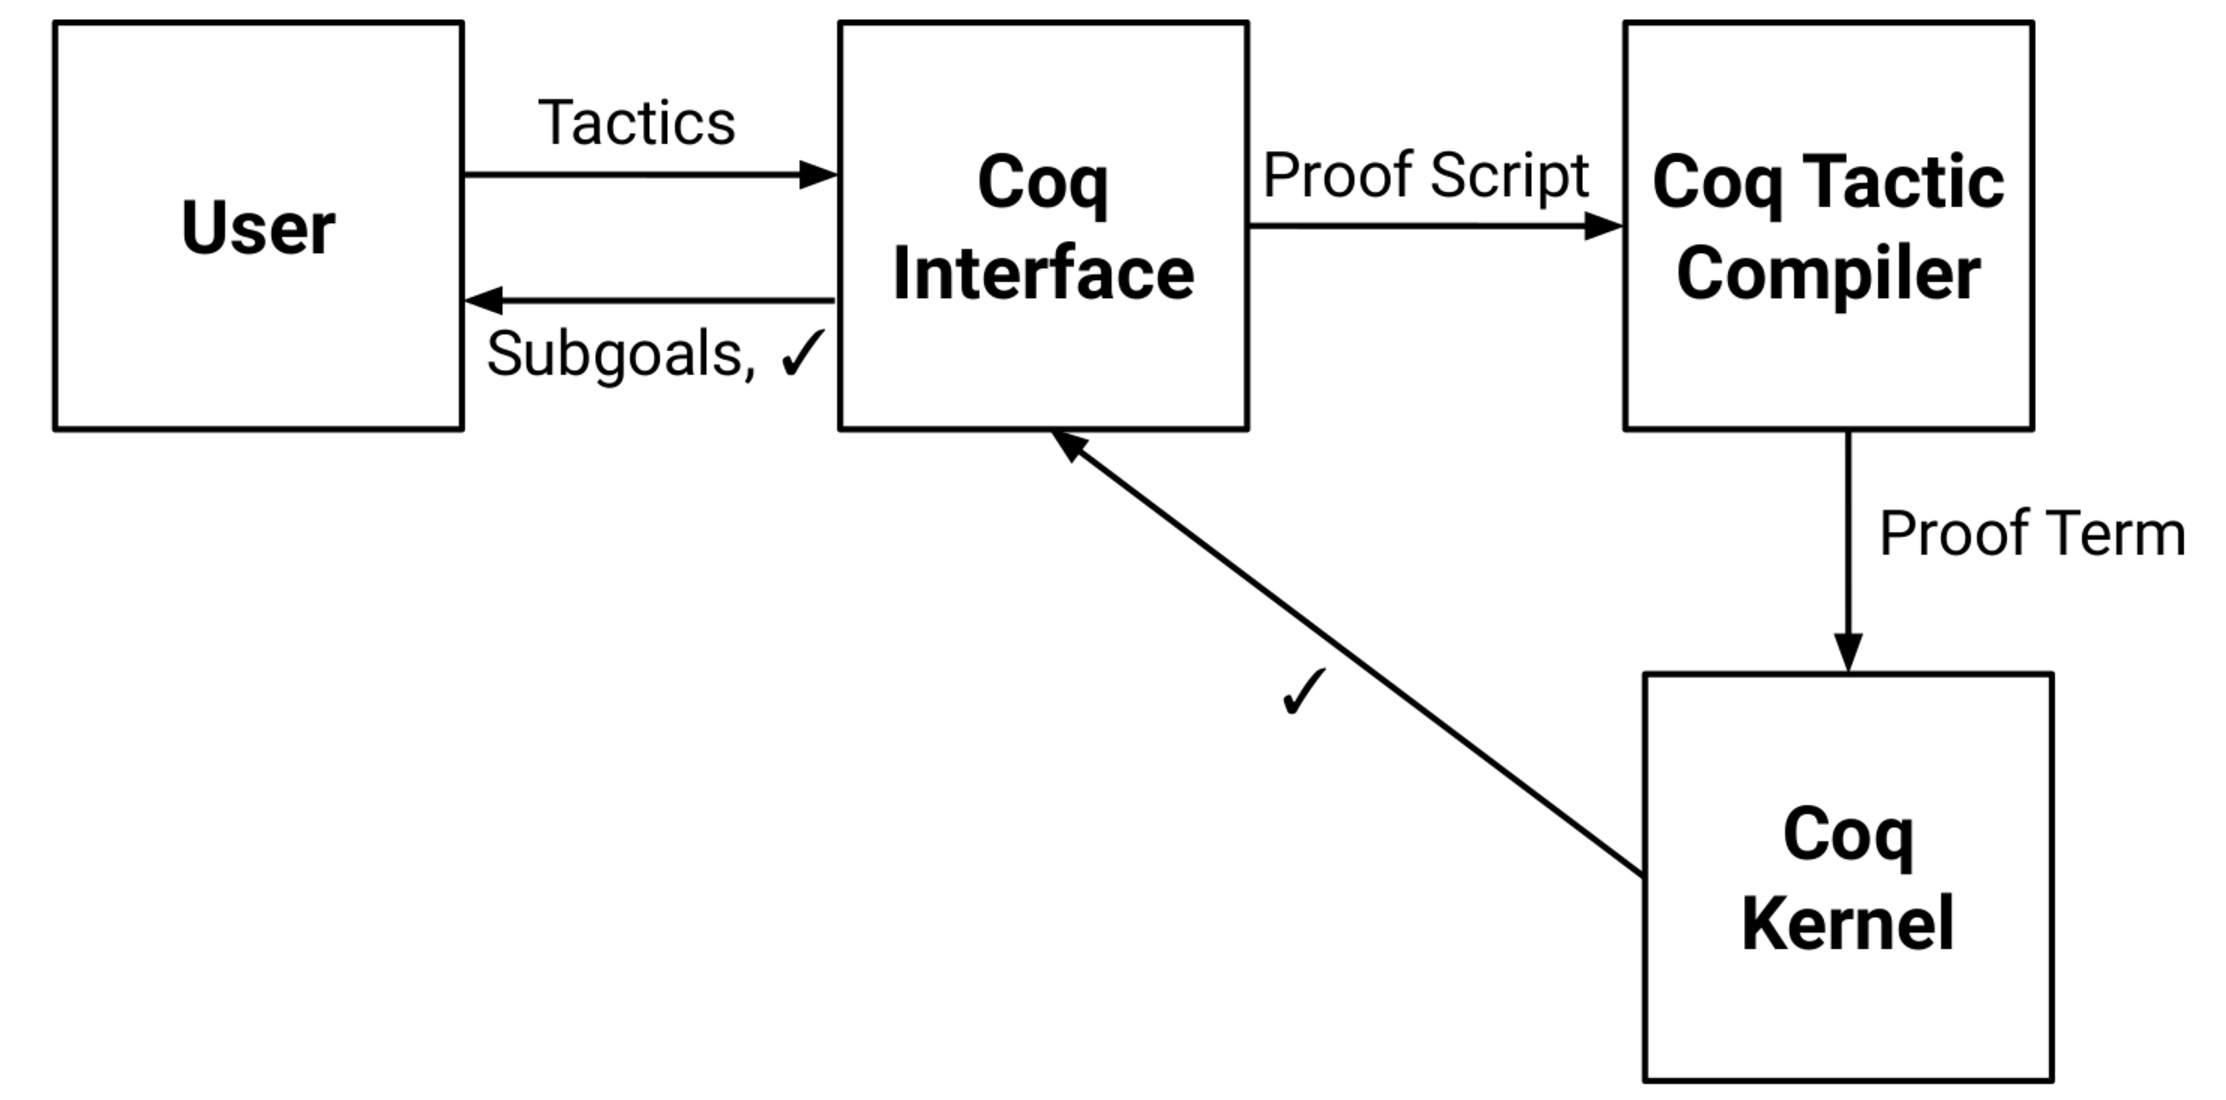
\includegraphics[scale=0.32]{Development}
\end{center}
\caption{An illustration of the typical interactive workflow of using the \kl{Coq} \kl{proof assistant} to write a proof. The checkmark at the end
represents correctness of the proof, which is communicated back to the proof engineer in the end.}
\label{fig:workflow}
\end{figure}

% TODO here, say: we assume Coq in here, see survey paper for more, tactics versus no tactics, de bruijn, where Coq is,
% many ideas generalize but eh, doesn't adapt exactly as-is.
% then expand on that in related work or conclusion

% TODO the amount of background: in reading guide, give resources for learning Coq in more detail, but don't go into too much Coq detail here

The way that proof engineers typically write proofs can obfuscate the information that changes in programs, specifications, and proofs carry.
The typical proof engineering workflow in \kl{Coq} is interactive: The proof engineer passes Coq high-level
search procedures called \textit{tactics} (like \lstinline{induction}), and Coq responds to each tactic
by refining the current goal to some subgoal (like the proof obligation for the base case). This loop of tactics and goals 
continues until no goals remain, at which point the proof engineer has constructed a high-level sequence of tactics called a \textit{proof script}.
To check the proof, Coq compiles it down to a low-level representation called a \textit{proof term},
then checks that the proof term has the expected type.
Figure~\ref{fig:workflow} illustrates this workflow.

The high-level language of tactics can abstract away important details that a proof repair tool needs,
but the low-level language of proof terms can be brittle and challenging to work with.
Crucially, though, the low-level language comes with lots of structure and strong guarantees.
My approach to proof repair works in the low-level language to take advantage of that.
It then builds back up to the high-level language in the end.

By working at the low-level language, it is able to systematically and with strong guarantees extract and generalize the 
information that breaking changes carry,
then apply those changes to fix other proofs broken by the same change.
But by later building up to the high-level language,
it can in the end produce proofs that integrate more naturally with proof engineering workflows.

This works using a combination of semantic differencing and program transformations in this low-level language.
In particular, it uses a semantic differencing algorithm to extract information from a breaking change in a program, specification, or proof.
It then combines that with program transformations to generalize and, in some cases, apply that information to fix other 
proofs broken by the same change.
In the end, it uses a prototype decompiler to get from the low-level language back up to the high-level language,
so that proof engineers can continue to work in that language going forward. % TODO lol this sucks but whatever it's a first draft

\section{Results}
\label{sec:intro-results}

The technical results of this thesis are threefold:

\begin{enumerate}
\item the \textbf{design} of differencing algorithms \& program transformations for proof repair, 
\item an \textbf{implementation} of a proof repair tool suite, and
\item \textbf{case studies} to evaluate the tool suite on real proof repair scenarios.
\end{enumerate}
Viewing the thesis statement as a theorem, the proof is as follows: % TODO link to particular sections here

\begin{quote}
\textbf{Thesis Proof}: Changes in programs, specifications, and proofs carry information that a tool can extract, generalize, and apply to fix other proofs broken by the same change (by \textbf{design} and \textbf{implementation}). A tool that automates this can save work for proof engineers relative to reference manual repairs in practical use cases (by \textbf{case studies}).
\end{quote}

\paragraph{Design}
The design describes semantic differencing algorithms to extract information from breaking changes in verified systems,
along with proof term transformations to generalize and, in some cases, apply the information to fix proofs broken by the change. % TODO redundant but shitty first draft text so whatever
The semantic differencing algorithms compare the old and new versions of a changed term or type,
and from that find a diff that describes that information corresponding to that change;
the transformations then use that diff to transform some term to a more general fix.
The details vary by the class of change supported.
These design is guided heavily by foundational developments in dependent type theory;
the theory is sprinkle throughout as appropriate. % TODO may want to list or link to sections here
More details including limitations are in the corresponding chapters. % TODO link to those chapters

\paragraph{Implementation}
The implementation shows that in fact \textit{a tool} can extract and generalize the information that changes carry,
and then apply that information to fix other proofs broken by the same change.
This implementation comes in the form of a proof repair tool suite for Coq called \sysnamelong (Proof Updater Mechanically Passing Knowledge Into New Proofs, Assisting the Coq Hacker).
\sysnamelong implements two kinds of proof repair: proof repair by example (Chapter~\ref{ch:example}) % TODO implementation chapters instead
and proof repair across type equivalences (Chapter~\ref{chapt:pi}). % 8.9.1 
Notably, since all repairs that \sysnamelong produces are checked Coq in the end, \sysnamelong does not extend \textit{Trusted Computing Base} (TCB):
the set of unverified components that the correctnes of the proof development depends on~\cite{TODO}. % TODO not just cite by also make this way less shitty of a definition
In total, \sysnamelong is about 15000 lines of code implemented in OCaml.
These 15000 lines of code consist of three plugins and a library,
which together bridge the gap between the theory supported by design and the practical proof repair needed for the case studies.
Toward that end, five notable features include:

\begin{enumerate}
\item a preprocessing tool to support features in the implementation language missing from the theory,
\item a prototype decompiler from proof terms to proof scripts for better workflow integration,
\item optimizations for efficiency,
\item meaningful error messages for usability, and
\item additional automation for applying patches. 
\end{enumerate}
More details and other features are in the corresponding chapters. % TODO link to those chapters

\paragraph{Case Studies}
The case studies show that \sysnamelong can save work for proof engineers relative to 
reference manual repairs in practical use cases. % TODO link to corresponding chapters instead
In particular, the case studies in Chapter~\ref{ch:example} show retroactively that a prototype implementation of proof repair
by example could have saved work for proof engineers on major proof developments.
The case studies in Chapter~\ref{chapt:pi} show that proof repair across type equivalences can save
and in fact has already saved work for proof engineers in practical use cases.

\section{Reading Guide}
\label{sec:guide}

% Dan: Instead, I strongly advocate an explicit section in Chapter 1 that lays this all out for the reader: what prior publications are being leaned on, where does text from those reappear, and most importantly, where -- in explicit sections of forthcoming chapters -- are expanded explanations and additional data.  Voila, your thesis is now both a self-contained coherent document and a useful 'appendix' for people who have already read large parts of what is to follow.

This thesis assumes some background in \kl{proof engineering}, type theory, and (to a lesser extent) the \kl{Coq} \kl{proof assistant}. 
I strongly encourage readers of all backgrounds who would like more context to better understand this thesis
look to my survey paper on proof engineering~\cite{PGL-045}, which includes a detailed list of resources
and is available for free on my website: \url{https://dependenttyp.es}.

I recommend that readers with less background on proof engineering, dependent type theory, or the Coq proof assistant
take time to digest Chapter~\ref{chapt:mot} before moving on---though I recommend that even Coq experts read Chapter~\ref{chapt:mot}!
Chapters~\ref{ch:example} and~\ref{chapt:pi} get rather technical, so it is normal not to understand every detail,
though you may always contact me with questions.

\subsection*{Previously Published Material}

While this thesis is self-contained, it centers material from two previously published papers:

\begin{itemize}
\item \textbf{Talia Ringer}, Nathaniel Yazdani, John Leo, and Dan Grossman. \intro{Adapting Proof Automation to Adapt Proofs}~\cite{ringer2018adapting}. CPP 2018.
\item \textbf{Talia Ringer}, RanDair Porter, Nathaniel Yazdani, John Leo, and Dan Grossman. \intro{Proof Repair Across Type Equivalences}~\cite{Ringer2021}. PLDI 2021.
\end{itemize}
It also includes material from three other papers:

\begin{itemize}
\item \textbf{Talia Ringer}, Nathaniel Yazdani, John Leo, and Dan Grossman. \intro{Ornaments for Proof Reuse in Coq}~\cite{Ringer2019}. ITP 2019.
\item \textbf{Talia Ringer}, Alex Sanchez-Stern, Dan Grossman, and Sorin Lerner. \intro{\textsc{REPLica}: REPL Instrumentation for Coq Analysis}~\cite{replica}. CPP 2020.
\item \textbf{Talia Ringer}, Karl Palmskog, Ilya Sergey, Milos Gligoric, and Zachary Tatlock. \intro{QED at Large: A Survey of Engineering of Formally Verified Software}~\cite{PGL-045}. Foundations and Trends® in Programming Languages: Vol. 5: No. 2-3, pp 102-281. 2019. 
\end{itemize}
Below is a map from each of these papers to corresponding sections,
along with an explanation of what is new in this thesis and what is omitted.
All of these papers can be found for free on my website.

\paragraph{Adapting Proof Automation to Adapt Proofs}
The bulk of Chapter~\ref{ch:example} comes from this paper,
though the content is significantly reorganized and reframed.
The introducton and conclusion of Chapter~\ref{ch:example} are fresh content.
Sections~\ref{sec:pumpkin-approach}, \ref{sec:pumpkin-diff}, \ref{sec:pumpkin-trans}, and~\ref{sec:pumpkin-impl}
all include additions and elaborations not found in the original paper.
Chapter~\ref{sec:related} includes some related work from this paper,
and Chapter~\ref{chapt:conclusions} includes some future work from this paper.

\paragraph{Proof Repair Across Type Equivalences}
Parts of the introduction and Section~\ref{sec:mot-theory} come from this paper.
The bulk of Chapter~\ref{chapt:pi} comes from this paper,
though the content is likewise reorganized and reframed.
The conclusion of Chapter~\ref{chapt:pi} is fresh content.
Sections~\ref{sec:pi-approach}, \ref{sec:pi-diff}, \ref{sec:pi-trans}, and~\ref{sec:pi-implementation}
all include additions and elaborations not found in the original paper.
Chapter~\ref{sec:related} includes some related work from this paper,
and Chapter~\ref{chapt:conclusions} includes some future work from this paper.

\paragraph{Ornaments for Proof Reuse in Coq}
The example from Section~\ref{sec:mot-dev} comes from this paper, though most of the text is new.
Parts of Section~\ref{sec:mot-theory} also come from this paper.
Section~\ref{sec:pi-diff} uses a simplified version of the search algorithm from this paper as an example.
Section~\ref{sec:eval} includes the evaluation from this paper with additional context.
Chapter~\ref{sec:related} includes some related work from this paper.
This thesis retires the name of the tool from this paper (\textsc{Devoid})
and uses the name of the generalized version of the tool from \kl{Proof Repair Across Type Equivalences} (\toolnamec) in its place.

\paragraph{\textsc{REPLica}}
Section~\ref{sec:irl} includes a few samples of this paper, as does the abstract.

\paragraph{QED at Large}
Chapter~\ref{chapt:mot} includes a few samples of this paper.
Chapter~\ref{sec:related} includes a large amount of related work from this paper.

\subsubsection*{Authorship Statements}

The material in this thesis draws on work that I did with
four student and postdoctoral coauthors: \kl{Nathaniel Yazdani}, \kl{RanDair Porter}, \kl{Alex Sanchez-Stern},
and \intro{Karl Palmskog}.
Below is a summary of the contributions of each of those coauthors,
indexed for later reference.
The contributions of my faculty and professional coauthors---\intro{John Leo}, \kl{Dan Grossman}, \kl{Zach Tatlock},
\intro{Ilya Sergey}, \intro{Milos Gligoric}, and \intro{Sorin Lerner}---were of course also extremely valuable:

\paragraph{Nathaniel Yazdani}
I worked with \kl{Nate} starting from when he was an undergraduate student.
Nate contributed conceptually to all three proof repair papers his name appears on,
helped with a number of the case studies,
implemented important features on the critical path to success,
and did some of the writing about his contributions.
Nate's contributions include:

\begin{enumerate}
\item a tool for preprocessing proof developments into a format suitable for repair,
\item higher-order transformations for applying proof term transformations over entire libraries, and
\item a key early insight about equality.
\end{enumerate}
All three of these were necessary to scale proof repair to help real proof engineers in practical scenarios.

\paragraph{RanDair Porter}
\kl{RanDair} joined the project as an undergraduate.
RanDair implemented a prototype decompiler from proof terms to proof scripts,
and wrote a description of the behavior of the decompiler that I built on in the corresponding paper.
This decompiler was necessary for integrating proof repair tools with real proof engineering workflows,
and it continues to inspire exciting work to this day.

\paragraph{Alex Sanchez-Stern}
\kl{Alex} worked with me as a PhD student on a user study of proof engineers during my visit \kl{UCSD}.
Alex designed, implemented, deployed, and evaluated one of the two analyses in the user study paper.
He also helped substantially in building the infrastructure necessary to deploy the user study,
and wrote large sections of the paper.
The user study and paper would not have happened without Alex.

\paragraph{Karl Palmskog}
\kl{Karl} was a postdoctoral researcher when he joined me on the survey paper.
Karl wrote entire chapters of the survey paper.
I could not have written that paper without Karl.

\subsubsection*{Pronouns}

In this thesis, I use ``I'' to refer to work that I did as part of my thesis work,
even though of course no work happens in a vacuum.
I use the names of my coauthors like ``\kl{Nate}'' or ``\kl{RanDair}'' when referring to work that my coauthors did,
when I was operating primarily in an advisory role.
When I collaborated with my coauthors, I name them and myself, like ``\kl{Nate} and I,''
and then (when not ambiguous) I use ``we'' thereafter.
Throughout, I also use mathematical ``we'' to mean both myself and the reader.

When I discuss a rhetorical proof engineer who does not actually exist,
like ``the proof engineer,'' I always use ``she''---this is a small attempt
to seed the world with data that counteracts stereotypes. 
When preserving anonymity of a particular person, I always use singular ``they.''
Otherwise, I use the pronouns that the person prefers.




